\documentclass[12pt]{article}

\setlength{\parskip}{1ex}
\addtolength{\textwidth}{.78in}
\addtolength{\textheight}{.18in}
\setlength{\oddsidemargin}{.2in}
%\usepackage{showkeys}

\usepackage{booktabs}
\newcommand{\ra}[1]{\renewcommand{\arraystretch}{#1}}
\usepackage{algorithm}
\usepackage{algpseudocode}
\usepackage{graphicx,amsmath,amssymb,wrapfig,color,amsfonts}
\usepackage[section]{placeins}
%\usepackage{showkeys}
\usepackage{enumitem}
\usepackage{subfig}
%\usepackage[margin=0.5in]{geometry}

\newcommand{\SWE}{shallow water equations }
\newcommand{\onehalf}{\frac{1}{2}}
%\newcommand{\pr}[1]{\frac{\partial #1}{\partial m}}
\newcommand{\pr}[1]{{#1}_m}
\newcommand{\rhot}{\widetilde{\rho}}
\newcommand{\rhoh}{\widehat{\rho}}
\newcommand{\ut}{\widetilde{u}}
\newcommand{\uh}{\widehat{u}}
\newcommand{\wt}{\widetilde{w}}
\newcommand{\wh}{\widehat{w}}
\newcommand{\pt}{\widetilde{p}}
\newcommand{\ph}{\widehat{p}}
\newcommand{\htil}{\widetilde{h}}
\newcommand{\hh}{\widehat{h}}
\newcommand{\commentout}[1]{}
\DeclareMathAlphabet\mathbfcal{OMS}{cmsy}{b}{n}

\begin{document}
\date{}

\title{A state redistribution algorithm for finite volume schemes
on cut cell meshes}
\author{Marsha Berger\footnote{Courant Institute, New York University, 251 Mercer St.,
NY, NY 10012}  \hspace{1in} Andrew Giuliani $^*$}

\maketitle

\begin{abstract}
In this paper we develop a new technique, called \textit{state redistribution}, 
that allows the use of explicit time stepping when approximating
solutions to hyperbolic conservation laws on embedded boundary grids.  
State redistribution is a postprocessing technique applied after each time 
step or stage of the base finite volume scheme, using a time step
that is proportional to the volume of the full cells.  The idea is to 
stabilize the cut cells by temporarily merging them into larger, 
possibly overlapping, neighborhoods, 
then replacing the cut cell values with a stabilized value
that maintains conservation and accuracy.
We present examples of state redistribution using two base schemes:
MUSCL and a second order Method of Lines finite volume scheme. 
State redistribution is used to compute solutions to several 
standard test problems in gas dynamics on cut cell meshes, with both
smooth and discontinuous solutions. We show that our method does not 
reduce the accuracy of the base scheme and 
that it successfully captures shocks in a non-oscillatory manner.
\end{abstract}

\section{Introduction}\label{sec:intro}
Cut cell meshes to solve hyperbolic problems 
are increasingly prevalent due to the ease 
of grid generation for complicated geometries \cite{}. 
However the {\em small cell} problem is still an active area of research, and
a completely satisfactory solution has not yet been found.
The small cell problem can be explained as follows: explicit
finite volume schemes typically need to take a time step 
that is proportional to the mesh width in order to satisfy a CFL constraint for
stability. However cut cells can have volumes that are arbitrarily
smaller than the regular cells that would otherwise determine the stable time
step. Special algorthms are needed to prevent this restriction.

The most commonly used stabilization algorithm is called flux
redistribution \cite{chern:colella,vof:colella}. The main idea is illustrated below in two space
dimensions, for ease of notation.
The essential idea is to compute the 
flux update for a cut cell $i,j$ with volume $V_{i,j} < V_{\mbox{\em full}}$,
\begin{eqnarray*}
V_{i,j} Q_{i,j} ^{n+1} & = V_{i,j} Q_{i,j}^n  +  \Delta t \, \Sigma_k F_k \cdot l_{k}\\
                   & = V_{i,j} Q_{i,j}^n  +  \delta  M 
\end{eqnarray*}
Here, $V_{\mbox{\em full}}$ is the volume of a full uncut cell.
Instead of using the entire amount of the update in cell ${i,j}$, 
the cut cell only uses a fraction $\eta$ of it.  If the fraction $\eta$
is proportional to the cell's volume
fraction $V_{i,j}/V_{\mbox{\em full}}$, the update should be stable. 
To maintain conservation, the rest of the update ($1-\eta)\delta M$
is given to the cell's neighbors.  
There are more recent additional steps that make the distribution 
more robust and accurate. For example, the difference between a stable
non-conservative update and the conservative update is what is
redistributed (see \cite{} for details).
Flux redistribution has already been implemented for three dimensional
calculations due to its simplicity. However it is only first order
accurate at the cut cells.

Cell merging is most frequently the first idea people 
think of. It is conceptually simple, but 
we are not aware of any production codes that implement this in a fully
general, robust manner for complicated engineering geometries. 
The $h$-box method \cite{mjb-hel-rjl:hbox2,mjb-hel:hboxsimple}
is a second order accurate method at the cut cells. It extends the 
domain of dependence for the fluxes around a small cell in a 
special way that maintains stability by means of a cancellation
property. It  has not been extended to
three dimensions due to its complexity. 

In Schneiders et al \cite{shws:2011}, the authors make
some improvements to flux redistribution for viscous flow in moving
geometries. They introduce a
smooth cutoff function of cell size for when it is applied. They also
use a non-uniform weighting in the gradient stencil to avoid abrupt
changes, which can lead to oscillations in the solution. This is
especially important for moving geometries.

In \cite{BalajiMenon:2016}, the authors also tackle viscous flow, with a
third order accurate (or higher) approach. They use a cluster of cells,
akin to cell merging, but maintain each cell's identity. A high order
polynomial is fit to the cluster, and replaces the solution values in the
individual cells.  Our algorithm has a similar spirit to this, though the
details are very different. HARD TO UNDERSTAND WHAT THE DO

In \cite{May-Berger:JSC}, an implicit scheme was developed to
handle stability of the cut cells, and was combined with an 
explicit method for the full cells. In this work we will focus on 
two explicit methods, and make modification necessary for them accuracy 
on the cut cells.
Other approaches that have been proposed in the literature include
interpolation-based procedures, such as the mirror-cell method by Forrer
and Jeltsch \cite{article:FoJe98}, and a related ghost-fluid method by
Dadone and Grossman \cite{DadoneGrossman}.
There are also approaches based on finite difference schemes
\cite{SjogreenPetersson,MarcoBjorn}
and kinetic schemes \cite{Oksuzoglu:thesis,KeenKarni}.
However, since we are interested in methods
that preserve conservation we do not explore these alternatives further.

In this paper we propose a framework for a stabilization algorithm in
the spirit of flux redistribution (henceforth FRD). 
As with FRD, it is applied as a postprocessing
step, and is simple to implement. Cell updates on all cells are performed
in the usual way, followed by a postprocessing step based on the
conserved state variables, not on the fluxes.
Hence we call it {\em state redistribution} (SRD).


To set the stage, notice that cell merging itself can
be rewritten as a postprocessing step.
\commentout{
To take one step to update a finite volume approximation to
$u_t + u_x = 0$ we do the following:
\begin{itemize}
\setlength\itemsep{.2in}
\item
{\bf Finite Volume Step}\\
Take the usual finite volume step with fixed, regular  $\Delta t$ on all cells 
including the small cell:
\begin{equation}
\bar{u}_j = u_j^n - \frac{\Delta t}{h_j} \; (f_{j+1/2} - f_{j-1/2} ), 
\quad \forall j.
\label{eqn:fvupdate}
\end{equation}

\item
{\bf {\em Temporarily} Create Merged Cell}\\
Temporarily create the {\em merged} cell $\overline{u_M}$ consisting of the small cell $u_j$ and one
or both of its neighbors so that it the merged cell is of sufficient
size (to be discussed later).  For simplicity here we will merge 
only with the neighbor on the right,
\begin{equation}
\widehat{q_M} =  \frac{ h_k \bar{u}_k + h_{k+1} \bar{u}_{k+1} } {h_k +
h_{k+1}} .
\label{eqn:mergestep}
\end{equation}

\item
{\bf Compute Merge Cell Gradient }\\
There are several ways to do this. 
Two simple possibilities are 
\begin{equation}
\nabla \widehat{u_M} = \frac{\bar{u}_{k+2} - \bar{u}_{k-1}} {x_{k+2}-x_{k-1}}
\label{eqn:gradLim1}
\end{equation}
which does not use the merged cell,
or
\begin{equation}
\nabla \widehat{u_M} = \frac{\bar{q}_{k+2} - \widehat{u_{M}}} {x_{k+2}-x_{M}}
\label{eqn:gradLim2}
\end{equation}
which uses the merged cell, and $x_M$ is the centroid of the merged
cell.
The choice of gradient stencil will be studied later in section \ref{sec:srdAlg}.

%Other more accurate alternatives exist, not all of which are stable.
%It would be better to use smaller stencils, perhaps including $u_{k+1}$
%or $\overline{u_M}$ itself.

\item
{\bf Redistribute Merged State to Cells Comprising Merged cell }\\
Replace the provisional values computed in the cells comprising the
merged cell with the merged solution reconstructed to the cell
centroids:
\begin{equation}
\begin{split}
u_k^{n+1} &= \widehat{u_M} +  (x_k - x_M) \nabla \widehat{u_M}\\
u_{k+1}^{n+1} &= \widehat{u_M} +  (x_{k+1} - x_M) \nabla \widehat{u_M}
\end{split}
\end{equation}
\end{itemize}
}
First  update cells $k$ and $k+1$, shown in Figure \ref{fig:modelProblem1},  using a standard finite volume scheme
with fixed $\Delta t$ on all cells:
\begin{equation}
\bar{u}_j = u_j^n - \frac{\Delta t}{h_j} \; (f_{j+1/2} - f_{j-1/2} ), 
\quad \forall j.
\label{eqn:fvupdate}
\end{equation}
Next form the merged cell
\begin{equation}
\widehat{q_M} =  \frac{ h_k \bar{u}_k + h_{k+1} \bar{u}_{k+1} } {h_k +
h_{k+1}} .
\label{eqn:mergestep}
\end{equation}
which works out to
\begin{equation}
\widehat{q_M} = \widehat{q_M}^n - 
\frac{\Delta t}{h_k + h_{k+1}} (f_{k+3/2} - f_{k-1/2})
\end{equation}

\begin{figure}
\begin{center}
%\vspace*{-.5in}
\includegraphics[height=1.3in]{figs/1dfig.pdf}
\caption{\sf Notation for model problem in one space dimension. The small
cell has size $\alpha h$ in a mesh with regular mesh width $h$.}
\label{fig:modelProblem1}
\end{center}
\end{figure}


For the simplest first order version, we simply set
\begin{equation}
u_k^{n+1} = u_{k+1}^{n+1} = \widehat{q_M}^{n+1} 
\label{eqn:finalstep}
\end{equation}
Recognizing that $h_k+h_{k+1}$ is the merged cell volume makes 
clear the relationship to cell merging.
If the final update step \eqref{eqn:finalstep}  is replaced by 
\begin{equation}
\begin{split}
u_k^{n+1} &= \widehat{q_M} +  (x_k - \widehat{x}_M) \,\, \nabla \widehat{q_M}\\
u_{k+1}^{n+1} &= \widehat{q_M} +  (x_{k+1} - \widehat{x}_M) \, \nabla \widehat{q_M}
\end{split}
\end{equation}
then the method is linearity preserving, 
if all gradients are computed accurately enough to preserve a linear function.  

By using a higher than linear polynomial and
including more neighbors in the
redistribution (on top of a more accurate finite volume scheme for the
entire mes ),
we have a path to higher order accuracy.
The method is also conservative since the mass of the merged cell equals the 
mass of the two cells comprising it.



The choice of merging neighborhoods and gradients is what makes up the
specifics of SRD in two space dimensions. Furthermore, it can happen
that a cell has more than one neighborhood with
which it should merge. This is what often causes complications in cell
merging algorithms. In SRD, we will simply use all such values appropriately
weighted.

In the next section  we first review the finite volume schemes to which SRD will
be applied.
The SRD algorithm in two space dimensions will be presented in section
\ref{sec:srdAlg}.
For simplicity we present the second order accurate version first.
The more general higher order extension is described in 
section \ref{sec:ho}.
Some theoretical results using one-dimensional model problems are in
section \ref{sec:theory}. 
Section \ref{sec:compResults} shows computational results for both smooth
problems and shocked flow for both linear advection and the Euler equations.  We conclude in section \ref{sec:conc}.

\section{State redistribution in one dimension} \label{sec:srd1d}
We begin this section  by reminding the reader that cell merging can
be written as a postprocessing step. We then show that the extension of
cell merging for overlapping cells does not maintain conservation. 
This motivates our state redistribution approach, which we contrast with
cell merging on a simple one dimensional example. 
Although the small cells do not mimic the cut cells at the 
boundary in higher dimensions, this is still a useful model problem. 

For the examples in this section we will solve the linear advection equation
\begin{equation}\label{eq:hpde}
u_t + au_x = 0, \quad a>0
\end{equation}
on the nonuniform grid, called the base grid. Equation \eqref{eq:hpde} is
discretized  using the  first order
accurate upwind scheme 
\begin{equation}\label{eq:unstable1d}
\widehat{U}_i = U^n_i - \frac{a \Delta t} {h_i} \, (U^n_i -U^n_{i-1}),
\end{equation}
where $U^n_i$ is the solution average on cell $i$ at time $t^n$, the time
step $\Delta t$ is constant for all cells. On full cells $h_i = h$, and on
the small cells  $h_i = \alpha h$ for $ 0 < \alpha < 1$.
We first use
the grid in Figure \ref{fig:ng1}(a) with one small cell at $i=0$, then the grid
in Figure \ref{fig:ng1}(b) with two small cells at $i = -1$ and $1$.

\begin{figure}[h]
\centering
\vspace*{.2in}
\mbox{
\includegraphics[width=0.4\linewidth,trim=30 0 20 0,clip]{figs/overlapping_simple.pdf} 
\hspace*{.1in}
\includegraphics[width=0.5\linewidth,trim=15 0 25 0,clip]{figs/overlapping.pdf}
}
\vspace*{.1in}
\caption{\sf Model problem in one space dimension on nonuniform base grid.
On the left there is one small cell at $i=0$. The right grid has two small 
cells  at $i = -1$ and $1$.  The small and large cell 
sizes are $\alpha h$ ($0<\alpha < 1$), and $h$, respectively. \label{fig:ng1}}
\end{figure}

On the grid in Figure \ref{fig:ng1}(a), cell merging might 
group cells -1,0, and 1 together into a larger, merged cell.
After the unstable update in \eqref{eq:unstable1d}, the  volume-weighted
merged cell average $\widehat{Q}_0$ is computed:
\begin{equation}
\widehat{Q}_0 = \frac{\widehat{U}_{-1} + \alpha \,  \widehat{U}_0 + 
\widehat{U}_1}{2+\alpha} .
\end{equation}
The cells comprising the merged cell
are then replaced by $\widehat{Q}_0$:
\begin{equation}
\widehat{U}_{-1}^{n+1} = \widehat{U}_0^{n+1} = \widehat{U}_1^{n+1} =
\widehat{Q}_0
\end{equation}
This is easily seen to be conservative by checking that
\begin{equation}
\underbrace{h \, (U_{-1}^{n+1} + \alpha \, U_0^{n+1} +
U_1^{n+1})}_{\text{mass after redistribution}}
= (2+\alpha) h \,  \, \widehat{Q}_0 =
\underbrace{ h \, (\widehat{U}_{-1} + \alpha \, \widehat{U}_{0} +
\widehat{U}_{1})}_{\text{mass before redistribution}}
\end{equation}
which equals the values at time $t^n$  except for the mass entering and
leaving this region.


Next, consider the more complicated case of Figure \ref{fig:ng1}(b).
Five cells (indexed by $-3$, $-2$, $0$, $2$, $3$) are large 
with size $h$ and the remaining two cells (indexed by $-1$ and $1$) 
are small with size $\alpha h$.
A first approach to cell merging on this grid
might be to make two merged cell averages, $\widehat{Q}_{-1}$
comprising cells ${-2},{-1},0$, and $\widehat{Q}_1$ comprising cells
$0, 1$ and $2$, associated respectively with the small cells $-1$ and $1$.
The first order version here would assign cells as before, except that
since cell 0 belongs to two neighborhoods, it seems  reasonable
to assign $U_0^{n+1} = \frac{1}{2} (\widehat{Q}_{-1} + \widehat{Q}_1).$  
To check for conservation, we again compute the sum
\begin{equation}
\begin{split}
\underbrace{h \, (U_{-2}^{n+1} + \alpha\,U_{-1}^{n+1} + U_0^{n+1} + \alpha \, U_1^{n+1}
+ U_2^{n+1})}_{\text{mass after redistribution}} = \\[.1in]
h \left [(1+\alpha +1/2) \, \widehat{Q}_{-1} +
 (1/2+\alpha +1) \, \widehat{Q}_{1}\right ]  = \\[.1in]
h \,  (3/2+\alpha) \, \left [ \frac{(\widehat{U}_{-2} + \alpha \widehat{U}_{-1} +
\widehat{U}_0)}{2+\alpha} +
        \frac{(\widehat{U}_{0} + \alpha \widehat{U}_{1} 
        + \widehat{U}_2)}{2+\alpha} \right ]  \neq \\[.08in]
\underbrace{h \,  ( \widehat{U}_{-2} + \alpha \widehat{U}_{-1} +
\widehat{U}_0 +  \alpha \widehat{U}_{1} + 
\widehat{U}_2 )}_{\text{mass before redistribution}}.  
\end{split}
\end{equation}
So at least this extension of cell merging to overlapping cells is not
conservative.

This motivates the state redistribution
procedure, which allows for overlapping cells and stabilizes 
$\widehat{U}_i$ in a conservative manner.
This is done by temporarily merging cells of the grid into 
larger, possibly overlapping, neighborhoods using a specially weighted 
convex combination, and recombining these averages back onto the
grid in a particular fashion.  These merged cells are 
constructed once during a mesh preprocessing step before time stepping.

\begin{figure}[h]
\begin{center}
\vspace*{.1in}
\includegraphics[width=0.75\linewidth]{figs/overlapping1.pdf} 
\caption{\sf 
The blue arrows indicate the merging neighborhoods associated with the large 
cells $-3$, $-2$, $0$, $2$, and $3$, which are their own neighborhoods.  
The red arrows indicate the neighborhoods of small cells $-1$ and $1$, which
have temporarily merged with their left and right neighbors.  
%The numbers next to the arrows are the neighborhood index, which
%correspond to the cell indices in Fig. \ref{fig:ng1}.  
\label{fig:mn1}}
\end{center}
\end{figure}

\subsubsection*{State redistribution preprocessing}
Each cell in the base grid (both large and small) has a merging neighborhood
associated with it.
This is  a set of neighboring cells with which to temporarily merge.
Neighborhoods share the same index as the cell that generated it.
%The merging neighborhood associated with cell $i$ is called $M_i$. 
Small cells merge with their neighbors until the volume of the merging neighborhood is greater than
a threshold, taken here to be half the large cell size of $h/2$.
This is illustrated by the red arrows in Figure \ref{fig:mn1} where the merging neighborhood of 
small cell $-1$ consists of cells $-2$, $-1$, and $0$, and the merging neighborhood of 
small cell 1 consists of cells $0$, $1$, and $2$. 
Note that   both neighborhoods overlap on cell 0. Allowing
for overlaps makes this temporary merging process simpler.
A large cell does not need to merge with neighbors (since $h > h/2$), thus its merging neighborhood is only 
composed of itself.  This is illustrated by the blue arrows in Figure
\ref{fig:mn1}. For example,  the 
merging neighborhood of large cell $-3$ is composed only of itself.

Finally, each cell in the base grid counts the number of neighborhoods that overlap it. 
Cell $-2$ is overlapped by two neighborhoods, indexed by $-1$ and $-2$.
Cell 0 has 3 such neighborhoods, its own, and one from each small cell adjacent to it.

\subsubsection*{State redistribution postprocessing}
Using the above information we can now stabilize \eqref{eq:unstable1d} using the state redistribution 
method on the grid in Figure \ref{fig:ng1}b.  
On each merging neighborhood, we compute a weighted solution average $\widehat Q_i$, where $i$ is the 
index of the merging neighborhood. 
$\widehat Q_i$ is computed by a convex combination of the averages $\widehat{U}_i$ of cells contained in the 
merging neighborhood, weighted by the inverse of its overlap count. 
For example, on merging neighborhood $-1$, the weighted solution average is
\begin{equation}\label{eq:neigh2}
\widehat{Q}_{-1} = \frac{1}{\underbrace{h/2 + \alpha h + h/3}_{\text{weighted volume}}}\biggr( \underbrace{\frac{h}{2} \widehat{U}_{-2} + \alpha h \widehat{U}_{-1} + \frac{h}{3}\widehat{U}_{0}}_{\text{weighted mass}} \biggr).
\end{equation}
In formula \eqref{eq:neigh2}  for the weighted mass,
the cell volume is divided by the number of neighborhoods that overlap the associated cell 
in the base grid. 
For example, the multiplier in front of $\widehat{U}_{-2}$ is $\frac{h}{2}$ since there are 
two neighborhoods (from cells $-1$ and $-2$) that overlap cell $-2$.  
Similarly, the multiplier in front of $\widehat{U}_{-1}$ is $\alpha h$ since there is only 
one neighborhood (its own) that overlaps cell $-1$.
Finally, the multiplier in front of $\widehat{U}_{0}$ is $\frac{h}{3}$ since there are three neighborhoods that overlap cell $0$, i.e., cell $0$ is overlapped by neighborhoods $-1$, $1$, and $0$.
These multipliers are then divided by the weighted volume,  $(h/2 + \alpha h + h/3)$.
i%since $\widehat{Q}_{-1} $ must be a convex combination of $\widehat{U}_{-2}$, $\widehat{U}_{-1}$, and $\widehat{U}_{0}$.
The weighted solution average on merging neighborhood $1$ is similarly defined as
\begin{equation}\label{eq:neigh3}
\widehat{Q}_{1} = \frac{1}{h/2 + \alpha h + h/3}\left( \frac{h}{2} \widehat{U}_{2} + \alpha h \widehat{U}_{1} + \frac{h}{3}\widehat{U}_{0} \right).
\end{equation}
The weighted solution averages on merging neighborhoods that contain only one cell are simply 
\begin{equation}\label{eq:neigh1}
\widehat{Q}_i = \widehat{U}_i \quad \text{ for } i = -3,-2,0,2,3.
\end{equation}

The stabilized solution average at time $t^{n+1}$ on a cell in the base grid is then 
given by the average of all the weighted neighborhood averages that overlap it.  
On the cell overlapped by three neighborhoods we have
\begin{equation} \label{eq:threeneigh}
U^{n+1}_{0} = \frac{1}{3}(\widehat{Q}_{-1}+\widehat{Q}_{0}+\widehat{Q}_{1}).
\end{equation}
On the  cells overlapped by two neighborhoods, we have
\begin{equation} \label{eq:twoneigh}
U^{n+1}_{-2} = \frac{1}{2}(\widehat{Q}_{-1}+\widehat{Q}_{-2}) \text{ and } U^{n+1}_{2} = \frac{1}{2}(\widehat{Q}_{1}+\widehat{Q}_{2}).
\end{equation}
Finally, on cells overlapped by only one neighborhood,  we have
\begin{equation} \label{eq:oneneigh}
	U^{n+1}_i = \widehat{Q}_i \text{ for } i = -3,-1,1,3.
\end{equation}

We can write the final solution update on the small cells after SRD  at $t^{n+1}$ in terms of the solution 
averages at $t^{n}$, giving
\begin{equation}
\begin{aligned}
U^{n+1}_{-1} &= \frac{2-2\lambda}{5+6\alpha}U^n_0 + \frac{6\alpha - 4 \lambda}{5+6\alpha}U^n_{i-1}+ \frac{3\lambda + 3}{5+6\alpha}U^n_{i-2}+\frac{3\lambda }{5+6\alpha}U^n_{i-3}, \\
U^{n+1}_{1} &= \frac{2+4\lambda}{5+6\alpha}U^n_0 + \frac{6\alpha - 3 \lambda}{5+6\alpha}U^n_{i+1}+ \frac{3-3\lambda}{5+6\alpha}U^n_{i+2}+\frac{2\lambda }{5+6\alpha}U^n_{i-1}.
\end{aligned} \label{eq:finalupdate}
\end{equation}
Before application of the state redistribution method, the weights that multiply the solution averages at time $t^n$ in the base scheme \eqref{eq:unstable1d} become unbounded as $\alpha \rightarrow 0$.
However, after state redistribution this is no longer the case for the weights 
in \eqref{eq:finalupdate}.  This hints at the stability of our modified scheme.  

The state redistribution algorithm allows us to take full time steps as if there were no 
small cells in the grid.  However, it can be seen that the multipliers of $U^n_{i-1}$ and $U^n_{i+1}$ 
in \eqref{eq:finalupdate} are negative when $\alpha$ is small enough.  This means that our scheme is not 
monotone and thus not total variation diminishing.  We note that this is also the case 
with flux redistribution, which has been successfully used in higher dimensions and more
complicated problems.  
The computational examples in Section \ref{sec:compResults} show that
this is not a significant issue for SRD as well.
The advantage of state redistribution  is that it is linearity
preserving, and flux redistribution is not. 

\subsubsection*{Conservation}
We now show that our modified scheme \eqref{eq:threeneigh}, \eqref{eq:twoneigh}, \eqref{eq:oneneigh} conserves mass.
%, i.e., the total mass of the numerical solution before and after state redistribution is the same.  
For the portion of the grid in question, the total mass after state redistribution is
\begin{equation}\label{eq:tm1}
	\sum_{i} h_i U^{n+1}_i  = h U^{n+1}_{-3} + h U^{n+1}_{-2} + \alpha h U^{n+1}_{-1} +h U^{n+1}_0+\alpha h U^{n+1}_{1} + h U^{n+1}_{2} + h U^{n+1}_{3},
\end{equation}
where $h_i$ is the local cell size.
%i.e., $h_i = \alpha h$ for $i \neq -1,1$ and $h_i = h$ otherwise.
Substituting expressions for the final update \eqref{eq:threeneigh}, \eqref{eq:twoneigh}, \eqref{eq:oneneigh} into \eqref{eq:tm1}, we obtain
\begin{equation}\label{eq:tm2}
\begin{aligned}
\sum_{i} h_i U^{n+1}_i  &= h \widehat{Q}_{-3} + \frac{h}{2}(\widehat{Q}_{-1}+\widehat{Q}_{-2}) \\
&+ \alpha h \widehat{Q}_{-1} +h \frac{1}{3}(\widehat{Q}_{-1}+\widehat{Q}_{0}+\widehat{Q}_{1})+\alpha h \widehat{Q}_{1} \\
&+ h \frac{1}{2}(\widehat{Q}_{1}+\widehat{Q}_{2}) + h \widehat{Q}_{3}.
\end{aligned}
\end{equation}
Grouping terms in \eqref{eq:tm2}, we have
\begin{equation}\label{eq:tm3}
\begin{aligned}
\sum_{i} h_i U^{n+1}_i  &= h \widehat{Q}_{-3} + \frac{h}{2}\widehat{Q}_{-2} \\
&+ \left(\frac{h}{2}+\alpha h + \frac{h}{3}\right) \widehat{Q}_{-1} + \frac{h}{3} \widehat{Q}_0 + \left(\frac{h}{2}+\alpha h + \frac{h}{3}\right) \widehat{Q}_{1} \\
&+ \frac{h}{2}\widehat{Q}_{2} + h \widehat{Q}_3.
\end{aligned}
\end{equation}
Substituting the expressions for the neighborhood averages \eqref{eq:neigh3}, \eqref{eq:neigh2}, \eqref{eq:neigh1} into \eqref{eq:tm3}, we obtain
\begin{equation}\label{eq:tm4}
\begin{aligned}
\sum_{i} h_i U^{n+1}_i  &= h \widehat{U}_{-3} + \frac{h}{2}\widehat{U}_{-2} \\
&+ \left(\frac{h}{2} \widehat{U}_{-2} + \alpha h \widehat{U}_{-1} + \frac{h}{3}\widehat{U}_{0}\right) + \frac{h}{3} \widehat{U}_0 + \left(\frac{h}{2} \widehat{U}_{2} + \alpha h \widehat{U}_{1} + \frac{h}{3}\widehat{U}_{0}\right) \\
&+ \frac{h}{2}\widehat{U}_{2} + h \widehat{U}_3.
\end{aligned}
\end{equation}
Simplifying \eqref{eq:tm4}, the mass after state redistribution becomes
\begin{equation}\label{eq:tm5}
\begin{aligned}
\sum_{i} h_i U^{n+1}_i  &= h \widehat{U}_{-3} + h \widehat{U}_{-2} + \alpha h \widehat{U}_{-1} +h \widehat{U}_0+\alpha h \widehat{U}_{1} + h \widehat{U}_{2} + h \widehat{U}_{3},\\
&= \sum_{i} h_i \widehat{U}_i.
\end{aligned}
\end{equation}
Thus, the mass on the grid before and after state redistribution does not change.
Since the base scheme \eqref{eq:unstable1d} is conservative, it follows from
\eqref{eq:tm5} that our modified scheme \eqref{eq:threeneigh},
\eqref{eq:twoneigh}, \eqref{eq:oneneigh} is too.
%, our modified scheme \eqref{eq:threeneigh}, \eqref{eq:twoneigh}, \eqref{eq:oneneigh} is conservative.  
%Thus, the base scheme coupled with the state redistribution method is conservative.  




The stabilized finite volume method \eqref{eq:threeneigh},
\eqref{eq:twoneigh}, \eqref{eq:oneneigh} is first order accurate in space
and time.  In this work, we provide a framework to generalize the state
redistribution method to two dimensional cut cell grids and to 
second order accuracy in space and time.
We will demonstrate with numerical examples that the maximum stable time step is 
not restricted by the small cells, and that the state redistribution method 
is conservative.



%In the next section  we discuss the base finite volume schemes that will be stabilized by state redistribution.


%\subsubsection*{Weighted volume of merging neighborhood}
%Each merging neighborhood has an associated a weighted volume




%\begin{equation}
%	\widehat{V}_i = \sum_{i \in M_i} \frac{h}{den}
%\end{equation}

%\subsubsection*{Solution average on merging neighborhood}
%We compute a weighted solution average on each merging neighborhood, $M_i$, using the following formula
%\begin{equation}\label{eq:merging}
%	\widehat{Q}_{i} = 
%\end{equation}



%The merging cell consists consisting of the small cell $u_j$ and one or both of its neighbors so that it the merged cell is of sufficient

%\begin{figure}
%	\subfloat[$50\times50$ grid and annulus domain.]{\includegraphics[width = 0.5\linewidth]{figs/rotatinghill_grid.eps} \label{fig:rotatinghillgrid}} 
%	\quad
%	\subfloat[Isolines of exact solution at the initial and final time. SHOW
%	COMPUTED SOLUTION TOO]{\includegraphics[width = 0.5\linewidth]{figs/rotatinghill_solution.eps}\label{fig:rotatinghillexactiso}}
%\end{figure}
%\begin{figure}
%	\begin{center}
%		%\vspace*{-.5in}
%		\includegraphics[height=1.3in]{figs/1dfig.pdf}
%		\caption{\sf Notation for model problem in one space dimension. The small
%			cell has size $\alpha h$ in a mesh with regular mesh width $h$.}
%		\label{fig:modelProblem1}
%	\end{center}
%\end{figure}


%To set the stage, notice that cell merging itself can
%be rewritten as a postprocessing step.
%\commentout{
%To take one step to update a finite volume approximation to
%$u_t + u_x = 0$ we do the following:
%\begin{itemize}
%\setlength\itemsep{.2in}
%\item
%{\bf Finite Volume Step}\\
%Take the usual finite volume step with fixed, regular  $\Delta t$ on all cells 
%including the small cell:
%\begin{equation}
%\bar{u}_j = u_j^n - \frac{\Delta t}{h_j} \; (f_{j+1/2} - f_{j-1/2} ), 
%\quad \forall j.
%\label{eqn:fvupdate}
%\end{equation}
%
%\item
%{\bf {\em Temporarily} Create Merged Cell}\\
%Temporarily create the {\em merged} cell $\overline{u_M}$ consisting of the small cell $u_j$ and one
%or both of its neighbors so that it the merged cell is of sufficient
%size (to be discussed later).  For simplicity here we will merge 
%only with the neighbor on the right,
%\begin{equation}
%\widehat{q_M} =  \frac{ h_k \bar{u}_k + h_{k+1} \bar{u}_{k+1} } {h_k +
%h_{k+1}} .
%\label{eqn:mergestep}
%\end{equation}
%
%\item
%{\bf Compute Merge Cell Gradient }\\
%There are several ways to do this. 
%Two simple possibilities are 
%\begin{equation}
%\nabla \widehat{u_M} = \frac{\bar{u}_{k+2} - \bar{u}_{k-1}} {x_{k+2}-x_{k-1}}
%\label{eqn:gradLim1}
%\end{equation}
%which does not use the merged cell,
%or
%\begin{equation}
%\nabla \widehat{u_M} = \frac{\bar{q}_{k+2} - \widehat{u_{M}}} {x_{k+2}-x_{M}}
%\label{eqn:gradLim2}
%\end{equation}
%which uses the merged cell, and $x_M$ is the centroid of the merged
%cell.
%The choice of gradient stencil will be studied later in section \ref{sec:srdAlg}.
%
%%Other more accurate alternatives exist, not all of which are stable.
%%It would be better to use smaller stencils, perhaps including $u_{k+1}$
%%or $\overline{u_M}$ itself.
%
%\item
%{\bf Redistribute Merged State to Cells Comprising Merged cell }\\
%Replace the provisional values computed in the cells comprising the
%merged cell with the merged solution reconstructed to the cell
%centroids:
%\begin{equation}
%\begin{split}
%u_k^{n+1} &= \widehat{u_M} +  (x_k - x_M) \nabla \widehat{u_M}\\
%u_{k+1}^{n+1} &= \widehat{u_M} +  (x_{k+1} - x_M) \nabla \widehat{u_M}
%\end{split}
%\end{equation}
%\end{itemize}
%}
%First update cells $k$ and $k+1$, shown in Figure \ref{fig:modelProblem1},  using a 
%standard finite volume scheme on all cells:
%\begin{equation}
%\bar{u}_j = u_j^n - \frac{\Delta t}{h_j} \; (f_{j+1/2} - f_{j-1/2} ), 
%\quad \forall j.
%\label{eqn:fvupdate}
%\end{equation}
%Next form the merged cell
%\begin{equation}
%\widehat{q_M} =  \frac{ h_k \bar{u}_k + h_{k+1} \bar{u}_{k+1} } {h_k +
%h_{k+1}} .
%\label{eqn:mergestep}
%\end{equation}
%which works out to
%\begin{equation}
%\widehat{q_M} = \widehat{q_M}^n - 
%\frac{\Delta t}{h_k + h_{k+1}} (f_{k+3/2} - f_{k-1/2})
%\end{equation}
%For the simplest first order version, we simply set
%\begin{equation}
%u_k^{n+1} = u_{k+1}^{n+1} = \widehat{q_M} 
%\label{eqn:finalstep}
%\end{equation}
%Recognizing that $h_k+h_{k+1}$ is the merged cell volume makes 
%clear the relationship to cell merging.
%The final update step \eqref{eqn:finalstep} is replaced by 
%\begin{equation}
%\begin{split}
%u_k^{n+1} &= \widehat{q_M} +  (x_k - \widehat{x}_M) \,\,  \widehat{\sigma_M}\\
%u_{k+1}^{n+1} &= \widehat{q_M} +  (x_{k+1} - \widehat{x}_M) \,  \widehat{\sigma_M}
%\end{split}
%\end{equation}
%where $\widehat{\sigma_M}$ is a reconstructed slope on the merged cell.
%The state redistribution method is linearity preserving when the base finite volume scheme and the reconstructed slope on merged cells $\widehat{\sigma_M}$ are accurate enough.
%By using a polynomial of degree $d>1$ and
%including more neighbors in the
%redistribution (on top of a more accurate finite volume scheme for the
%entire mesh),
%we have a path to higher order accuracy.
%The method is also conservative since the mass of the merged cell equals the 
%mass of the two cells comprising it.



%The choice of merging neighborhoods and gradients is what makes up the
%specifics of SRD in two space dimensions. Furthermore, it can happen
%that a cell has more than one neighborhood with
%which it should merge. This is what often causes complications in cell
%merging algorithms. In SRD, we will simply use all such values appropriately
%weighted.
%
%In the next section  we first discuss the finite volume schemes to which SRD will
%be applied.
%The SRD algorithm in two space dimensions will be presented in section
%\ref{sec:srdAlg}.
%For simplicity we present the second order accurate version first.
%The more general higher order extension is described in 
%section \ref{sec:ho}.
%Some theoretical results using one-dimensional model problems are in
%section \ref{sec:theory}. 
%Section \ref{sec:compResults} shows computational results for both smooth
%problems and shocked flow for both linear advection and the Euler equations.  We conclude in section \ref{sec:conc}.

\section{Second-Order Accurate Base Schemes}\label{sec:basefv}
We are interested in solving hyperbolic conservation laws 
\begin{equation}
\begin{aligned} \label{eq:conslaw2D}
\frac{\partial}{\partial t}	\mathbf{u} + \nabla \cdot \mathbfcal{F}(u)  = \mathbf{0}
\end{aligned}
\end{equation}
on the domain $\Omega \subset \mathbb{R}^2$ where $\mathbf{u}(x,y,t) \in \Omega \times (0,T]$ is a vector of conserved quantities, $T$ is the final time, and $\mathbfcal{F} = [\mathbf{F}, \mathbf{G}]$ is the flux function.  We discretize $\Omega$ into a cut cell mesh of cells $\Omega_{i,j}$.  A typical cut cell mesh, called the base grid, is given in Figure \ref{fig:2dfig}.  On the domain interior, the elements $\Omega_{i,j}$ are Cartesian cells (quadrilaterals) of size $\Delta x$ in the $x$ direction and $\Delta y$ in the $y$ direction.  On the domain boundary there is a border of irregular polygonal cells, called cut cells.  



There are two issues when applying an explicit finite volume scheme to a cut cell
mesh.  For accuracy, the scheme needs to be adapted in the cut cells. Second, 
the scheme needs to be stabilized in the cut cells if using a fixed timestep $\Delta t$ 
based on the full cells. In the $h$-box method these two concerns were addressed
simultaneously, but in general they aren't.

We will use two different second order discretizations of \eqref{eq:conslaw2D}: the method of lines
(MOL) approach and the MUSCL scheme.
These fully discrete finite volume methods, described in Section \ref{sec:mol} and \ref{sec:muscl},
are referred to as the base schemes.  Both schemes require linear 
reconstruction on grid cells,
outlined in Section \ref{sec:limit}.  The high-order extension of MOL and SRD  will be described 
in Appendix \ref{sec:ho}. Finally, both second order schemes evaluate the flux at
the boundary in the examples of Section \ref{sec:compResults} by extrapolating the
pressure to the boundary midpoint. Something more elaborate is done in the higher
order case. 

\begin{figure}
\begin{center}
\includegraphics[width=3.0in]{figs/example_ccmesh.pdf}
\caption{\sf Example base grid in two space dimensions. The cells shaded in yellow are the cut cells.  Both the method of lines (Section \ref{sec:mol}) and MUSCL (Section \ref{sec:muscl}) schemes require gradient information to reconstruct to the edge midpoint, indicated with a cross ($\times$).} 
\label{fig:2dfig}
\end{center}
\end{figure}


\subsection{Method of lines} \label{sec:mol}

After generating the cut cell mesh, we approximate the solution to \eqref{eq:conslaw2D} on this base grid using a finite volume method of the form
\begin{equation}\label{eq:fvscheme}
\frac{d}{dt}\mathbf{U}_{i,j} =- \frac{1}{V_{i,j}} \int_{\partial \Omega_{i,j}} \mathbfcal{F} ^* \cdot \mathbf{n} ~dl,
\end{equation}
where $\mathbf{U}_{i,j}$ is a vector of the cell averages on $\Omega_{i,j}$, $\partial \Omega_{i,j}$ is the cell boundary, $\mathbf{n}$ is an outward facing normal, and $\mathbfcal{F}^*$ is a numerical flux function.

Second order accuracy in space is achieved by reconstructing a gradient on each
cell and using it to evaluate the numerical flux at the face midpoints,
illustrated in Figure \ref{fig:2dfig}.  
In our numerical experiments, we use the local Lax-Friedrichs numerical flux to solve the Riemann 
problem at cell interfaces. The integral in \eqref{eq:fvscheme} is  approximated using the midpoint rule.

Second order accuracy in time is obtained by integrating \eqref{eq:fvscheme} using Heun's method.  This is a two-stage Runge Kutta method that can be written
\begin{equation}\label{eq:molscheme}
\begin{aligned}
	\mathbf{U}^{(1)} &= \mathbf{U}^{n} + \Delta t L(\mathbf{U}^n), \\
	\mathbf{U}^{(2)} &= \mathbf{U}^{(1)} + \Delta t L(\mathbf{U}^{(1)}), \\
	\mathbf{U}^{n+1} &= \frac{1}{2}( \mathbf{U}^{n} + \mathbf{U}^{(2)} ) ,	
\end{aligned}
\end{equation}
where $\mathbf{U}^{n}$ is the vector of solution averages on the entire cut cell mesh at time $t^n$,
$\mathbf{U}^{(1)}$,$\mathbf{U}^{(2)}$, are intermediate stages, and $L$ is the operator that results
from discretizing the right-hand-side of \eqref{eq:fvscheme}.
We derive the maximum stable time step on the base grid by using \eqref{eq:molscheme} to solve the linear advection equation on a Cartesian grid with advection velocity $(a,b)$.
Numerical evaluation of the amplification factor that results from a linear stability analysis reveals that a stable time step satisfies
\begin{equation}\label{eq:vn1}
\Delta t   \left( \frac{|a|}{\Delta x} + \frac{|b|}{\Delta y} \right)\leq 1.
\end{equation}
%We have verified \eqref{eq:vn1} by numerical evaluation of the amplification factor that results from a linear stability analysis.
Note that this is less restrictive than the time step required for a discrete maximum principle to be 
satisfied (see \cite{giuliani2018analysis}), which is 
\begin{equation}
\Delta t  \left( \frac{2\Delta x + 2 \Delta y}{\Delta x \Delta y} \right) \sqrt{a^2 + b^2}\leq 1 .
\end{equation}
%\begin{equation}
%\Delta t \,  \max\left(\frac{u}{\Delta x},\frac{v}{\Delta y}\right) \leq \frac{1}{2} ,
%\end{equation}
%For high order RK schemes, SRD is applied multiple times, before the final solution is assembled at the new time
%step. 
%With the Method of Lines scheme using SSP Runge Kutta time steppers, SRD is applied after each Forward Euler step. 
%If the Runge Kutta scheme is not SSP, SRD can be applied to each intermediate solution of the time stepper.
%If applied at the final stage, it does not need to be applied to the 
%resulting $U^{n+1}$.

For this method, we apply SRD stabilization to the stage updates
$U^{(1)}$ and $U^{(2)}$ in \eqref{eq:molscheme}, before they are added to form $U^{n+1}$.

\subsection{MUSCL scheme} \label{sec:muscl}
The MUSCL scheme is a one step method that is second order accurate in
space and time. A series of MUSCL schemes  was originated by van Leer 
\cite{vanleer:muscl}. The version we use\footnote{Thanks to Phil 
Colella for the original Cartesian mesh code and for helpful discussions on the shear
layer instability and artificial viscosity.}
is due to Colella \cite{Colella:Unsplit}.
The method is briefly sketched here so that we can describe how it was
adapted for cut cells. 

On a regular cell $(i,j)$ the interface values on the 
faces are computed at the half-step in time $t^{n+1/2}$, and the left and right states
are passed to a Riemann
solver to compute the fluxes.
Using a Taylor series in space and time to second order,
and using the conservation law \eqref{eq:conslaw2D}  to replace the derivative in time, gives the value for the right cell
interface $(i+1/2,j)$ 
%& = \mathbf{U}_{i,j}^n + 
%\frac{\Delta t}{2} \frac{\partial \mathbf{U}_{i,j}^n}{\partial t} + 
%\frac{\Delta x}{2} \frac{\partial \mathbf{U}_{i,j}^n}{\partial x} \\[.08in]
%&  = \mathbf{U}_{i,j}^n + \frac{\Delta t}{2} 
%\left(-\frac{\partial \mathbf{F}_{i,j}^n}{\partial x} -
%\frac{\partial \mathbf{G}_{i,j}^n}{\partial y} \right)  +
%\frac{\Delta x}{2} \, \frac{\partial \mathbf{U}_{i,j}^n}{\partial x} \\[.08in]
%&
\begin{equation}\label{eqn:taylor}
\begin{split}
\mathbf{U}_{i+1/2,j}^{n+1/2}    
              &= \mathbf{U}_{i,j}^n +  
\frac{\Delta t}{2} \frac{\partial \mathbf{U}_{i,j}^n}{\partial t} + 
\frac{\Delta x}{2} \frac{\partial \mathbf{U}_{i,j}^n}{\partial x} \\[.08in]
              &= \mathbf{U}_{i,j}^n - \frac{\Delta t}{2} \, 
             \frac{\partial \mathbf{G}_{i,j}^n}{\partial y}  -
            \left( \frac{\Delta t}{2} 
            \frac{\partial \mathbf{F}_{i,j}^n}{\partial \mathbf{U}^n_{i,j}} -
             \frac{\Delta x}{2} \right) \,\frac{\partial \mathbf{U}_{i,j}^n}{\partial x}, \\[.08in]
\end{split}
\end{equation}
The values at the other interfaces of full cells are similarly defined.


In the original method,
Riemann problems are solved in the transverse direction, e.g. between
centroids $(i,j)$ and $(i,j-1)$, at the edge $j-1/2$, to produce
$G_{i,j-1/2}$. 
The terms were then differenced to compute 
\begin{equation}
\partial G_{i,j}/\partial y =  (\mathbf{G}_{i,j+1/2} - \mathbf{G}_{i,j-1/2})/\Delta y .
\label{eqn:transdiff}
\end{equation}
On a uniform mesh 
the first order accurate errors in computing \eqref{eqn:transdiff} 
cancel, and the term itself is 
multiplied by $\Delta t$ in \eqref{eqn:taylor}.
For more details the reader is referred to \cite{Colella:Unsplit}.

At the cut cells the above procedure is no longer accurate,
since  the centroid values are not coordinate aligned near
the cut cells.
We make two modifications to the
computation of $\partial G/\partial y$, known as the
transverse derivative since it is in the vertical direction
when computing the flux $F$ in the horizontal direction.
First,
the solution is reconstructed in the transverse direction
to the edge midpoint so it is properly centered in cells that
are adjacent to a cut cell.  This is the situation
in Figure \ref{fig:2dfig} for cell $(i,j+1)$, for example.

Secondly, many cut cells will not have both edges in the
transverse ($y$) direction. Instead, for all cut cells we
instead compute
$ \partial \mathbf{G}_{i,j}^n / \partial y = ( \partial \mathbf{G}_{i,j}^n / \partial \mathbf{U}_{i,j}^n)( \partial \mathbf{U}_{i,j}^n / \partial y)$,
like the horizontal fluxes in \eqref{eqn:taylor}. This is linearly exact in the cut cells, 
if the gradients themselves are.
We also experimented with dropping this term in the cut cells
altogether. There was no stability problem with this, but it
does introduce an unnecessary difference from
the interior scheme, and would not be linearly exact.

\textit{Note:} it is the transverse derivative term that provides the so-called corner 
coupling, i.e. inclusion
of corner cells in the stencil. This is what  gives  the MUSCL scheme a linear stability limit of
\begin{equation}
\label{eqn:bigcfllimit}
\Delta t \, \max \left (\frac{|a|}{\Delta x} , \frac{|b|}{\Delta y} \right) \leq 1,
\end{equation}
where $(a,b)$ is the advection velocity.  

The trickiest term to adapt to cut cells was an artificial viscosity in the original method that was 
added to each flux, with a
coefficient proportional to the negative divergence of the flow.  The original
code used a large stencil to compute this divergence. We instead use a centered
difference to compute $u_x$ and $v_y$, and where possible, and  
take the max of this over a $3 \times  3$
neighborhood centered around each cell, so that cut cells get this dissipation too. 

\commentout{
As remarked above, it is the transverse derivatives that allows for the larger time
step given in \eqref{eqn:bigcfllimit}.
However, in the neighborhood of a shock the derivatives will be limited, and
possibly set to zero.
If these terms were not used  in the volume mesh, the time step would be reduced to 
\begin{equation}
\Delta t \, \left (\frac{u+c}{\Delta x} + \frac{v+c}{\Delta y} \right) < 1
\end{equation}
which could be as small as half the larger limit in eq. \eqref{eqn:bigcfllimit}.
However, as shown in \cite{mjb:stability2} for one space dimension, 
boundary cells can have
a local {\em cfl} number that is up to twice the stable {\em cfl} of the regular
mesh and the overall scheme remains stable.  We have not found any stability
problems due to limiting of this term.  
}

The multi-dimensional MUSCL scheme due to Colella has several additional
features to robustly handle strong shocks, such as not including terms in
predicting the interface state from characteristics that propagate 
away from the interface. These
steps do not change at the cut cells, so are not discussed here.  

Since MUSCL is a one-step scheme, the SRD stabilization is applied directly
before the final update
$\mathbf{U}^{n+1} = SRD(\mathbf{U}^{n} + \Delta t
L(\mathbf{U}^{n}))$, where $L$ is now the MUSCL operator.



\subsection{Gradient reconstruction and limiting }\label{sec:limit}

The computation of gradients, and for problems with discontinuities limiting
those gradients, arises independently of the finite volume scheme used. 
On the domain interior, when the stencil is regular and does not contain cut cells, standard schemes can be used.
In all our examples we use monotonized central (MC) differencing in both $x$ and $y$ directions.  The MC limited slope in the $x$ direction is
\begin{equation}
\sigma^n_{x,i,j} =  \begin{cases} 
\min \left ( \,  \lvert{ D_c}\rvert,\,
2 \lvert {D_+}\rvert,\,
2 \lvert{D_-}\rvert \,  \right ) \,\times 
\text{ sign } D_c, \quad \text{if} \;\;  D_+ D_- >  0,\\
0 \hspace*{2.8in} \text{otherwise}.
\end{cases}
\end{equation}
Here we use the standard differencing notation
$D_c = (U^n_{i+1,j}-U^n_{i-1,j})/(2 \, \Delta x)$ for the second order accurate central difference and
$D_+ = (U^n_{i+1,j}-U^n_{i,j})/\Delta x$,
$D_- = (U^n_{i,j}-U^n_{i-1,j})/\Delta x$ for the one-sided differences.  The MC limited slope in the $y$ direction is similarly defined.

For cut cells 
%and their neighboring full cells, 
we use a least squares gradient reconstruction algorithm, a standard procedure
for unstructured meshes.
%Cells that are two away from a cut cell can use any limiter with a five point stencil. 
A linear reconstruction of the solution on these cells is of the form
\begin{equation}
u^n_{i,j}(x,y) = U_{i,j}^n + \sigma^n_{x,i,j} \,(x-x_{i,j}) +
                     \sigma^n_{y,i,j}\,(y-y_{i,j}),
\label{eqn:lls}
\end{equation}
where $(i,j)$ is the index of either a cut cell or cell with an irregular stencil, $(\sigma^n_{x},\sigma^n_{y})_{i,j}$ and $(x,y)_{i,j}$ are its gradient and cell centroid, respectively. The least squares procedure finds the gradient that minimizes the $L_2$ residual when evaluating  $u_{i,j}(x,y)$ at  
neighboring cell centroids. 

In this work, we consider both first and second order accurate 
gradients.  The reconstructed first order gradient satisfies in the 
least squares sense
\begin{equation}\label{eqn:linrecon_base}
\sigma^n_{x,i,j}(x_{r,s} - x_{i,j}) +
\sigma^n_{y,i,j}(y_{r,s} - y_{i,j})=
U^n_{r,s} - U^n_{i, j} \quad \forall (r,s) \in R_{i,j},
\end{equation}
where $R_{i,j}$ is the set of cell indices used for slope reconstruction on cell $(i,j)$ in the 
base scheme.  Here, $R_{i,j}$ is the $3\times 3$ neighborhoood  centered on $(i,j)$.
The reconstructed second order gradient satisfies in the least squares sense
\begin{equation}
\begin{aligned}\label{eqn:linrecon_base2}
&\sigma^n_{x,i,j}(x_{r,s} - x_{i,j}) +
\sigma^n_{y,i,j}(y_{r,s} - y_{i,j})  + \\
&\quad \frac{1}{2}\sigma^n_{xx,i,j}[(x_{r,s} - x_{i,j})^2 - S_{xx,i,j}]  + \\
& \quad \; \sigma^n_{xy,i,j}[(x_{r,s} - x_{i,j})(y_{r,s} - y_{i,j})-S_{xy,i}] +\\
&\quad  \frac{1}{2}\sigma^n_{yy,i,j}[(y_{r,s} - y_{i,j})^2 - S_{yy,i,j}]
 \; = \;  U^n_{r,s} - U^n_{i, j} \quad \forall (r,s) \in R_{i,j},
\end{aligned}
\end{equation}
where $\sigma_{xx,i,j}$, $\sigma_{xy,i,j}$, $\sigma_{yy,i,j}$ are quadratic degrees of freedom and are discarded.  In this case, $R_{i,j}$ is either the $3\times 3$ tile centered on $(i,j)$ when $(i,j)$ is a whole cell neighboring a cut cell, or the $5\times 5$ tile centered on $(i,j)$ when $(i,j)$ is a a cut cell.
Note that a cut cell needs a larger neighborhood because 
approximately half of its cells are not in the flow domain.  

Regular cells that are adjacent to a cut cell will also need special treatment to
compute a second order accurate gradient. We have experimented with three  approaches
and found almost indistinguishable results. Simplest is to use the 
procedure mentioned above for cut cells
- fit a least squares polynomial in the $3 \times 3$ neighborhood centered on that cell.
We also tried $5 \times 5$ neighborhoods, in hope of smoother transitions between cut cells
and the interior cells.  Finally, we tried using a centered
gradient in only one dimension, if there was one, and using a recentering approach to 
compute the second order accurate difference in the other direction.  This has an overall
smaller stencil, but still uses the $3 \times 3$ if there is no regular direction,
and involves more testing.  

For problems with discontinuities, the gradient will need to be limited
to prevent overshoots and retain positivity for quantities like density and
pressure.
We use the Barth Jespersen (BJ)  limiter \cite{barth-jespersen} to limit on 
cut cell grids. 
This is a scalar limiter, where both $\sigma_{x,i,j}$ and $\sigma_{y,i,j}$ 
are reduced by the same scalar to prevent new extrema.  
We compute the minimum and maximum values over the reconstruction 
stencil $R_{i,j}$, 
\begin{equation} 
m_{i,j} = \max_{(r,s) \in R_{i,j}} U^n_{r,s} \text{ and } 
M_{i,j} = \max_{(r,s) \in R_{i,j}} U^n_{r,s}.
\label{eqn:bj1}
\end{equation}
The reconstructed gradient on cell $(i,j)$ is limited by a non-negative 
scalar $\alpha \in [0,1]$, so that when ${u}_{i,j}(x,y)$ 
is evaluated at the centroids of the neighborhoods in $R_{i,j}$ it
lies between $m_{i,j}$ and $M_{i,j}$.
(Apologies for reusing the symbol $\alpha$, since it is commonly 
used to describe Barth-Jespersen-type limiters, as well as the 
mesh width $\alpha h$  of small cells).

The limited numerical solution is
\begin{equation}
     \tilde{u}^n_{i,j}(x,y) = U_{i,j}^n + \alpha \, [{\sigma}^n_{x,i,j} ( x -  x_{i,j}) \, 
   + {\sigma}^n_{y,i,j}( y -  y_{i,j})].
\end{equation}
Define
\begin{equation}\label{eq:bj_alpha}
    \alpha_{r,s} = \begin{cases}
           \min \left(1,\frac{M_{i,j}-U_{i,j}^n}{U^n_{r,s} - U_{i,j}^n} \right)
    \quad  \text{ if } \,   U_{r,s}^n - U_{i,j}^n >  0,\\[.08in]
            \min \left(1, \frac{m_{i,j}-U_{i,j}^n}{U^n_{r,s} - U_{i,j}^n} \right)  
    \quad  \text{ if }  \, U^n_{r,s} - U_{i,j}^n < 0.\\[.08in]
             1    \hspace*{1.45in}  \text{if} \; \, U^n_{r,s} - U_{i,j}^n = 0.
    \end{cases}
\end{equation}
Then choose
\begin{equation}\label{eqn:alpha}
\alpha = \min_{(r,s) \in R_{i,j}} \alpha_{r,s} .
\end{equation}

By reconstructing to the neighboring cell centroids, this procedure is linearity preserving.  

The approach described above differs slightly from the original Barth-Jespersen limiter in
\cite{barth-jespersen}, where the numerical solution is reconstructed to 
points on cell interfaces.
This is often the procedure used on unstructured meshes. However cut cell meshes are much more
irregular and without this fix BJ can lead to much less accurate solutions.


\section{The State Redistribution Algorithm}\label{sec:srdAlg}

In this section we describe only the second order accurate version of the State
Redistribution Algorithm. 
This helps simplify the notation and make the
algorithm more intuitive.   
At several places there are choices
to make, and we discuss the alternatives and the reason behind our
choices.  Since the postprocessing step comes after the finite
volume update step, we begin this section by briefly reviewing the 
two methods that SRD is applied to.  

\subsection{The Base  Finite Volume Schemes}

Our computational results will use two different finite volume schemes
to update the Cartesian cut cell mesh.
We will refer to these at the base schemes. 
The  update is applied to the entire mesh, including  
to the small cut cells.  Since cut cells can have cell volumes that are
orders of magnitude smaller than the time step allowed by the full
cells, these will lead to instability without a stabilization algorithm.
SRD will be applied after each stage or step of the base scheme.

\begin{figure}
\begin{center}
\includegraphics[width=2.8in]{figs/2dfig.pdf}
\caption{\sf Notation for mesh in two space dimensions. The cells shaded
in yellow are the cut cells.} 
\label{fig:2dfig}
\end{center}
\end{figure}

\subsubsection{Method of Lines approach}
The simplest scheme is to use a spatial discretization over the entire
mesh, and apply a Runge-Kutta scheme in time. This is a well-known
standard approach
on regular Cartesian meshes. It is adapted for the cut cells by
using a least squares reconstruction of the gradient that includes
either edge and node neighbors (unless otherwise specified).
Limiting is done using the Barth-Jespersen limiter \cite{} 
on the cut cells and one adjacent neighbors. Any limiter
can be used for the regular cells.

The spatial reconstruction in the cut cells is no longer
coordinate-aligned, and is modified
to include both $x$ and $y$ components of the gradient to 
reconstruct to the midpoint of the cell edge. This is indicated 
in figure \ref{fig:2dfig}  with a green $\times$.
The SRD stabilization scheme is applied after each stage of
the Runge-Kutta scheme. 
Note that the time step restriction that results from the von Neumann stability analysis of this scheme applied to the linear advection equation is  (AG -
TRUE?)
\begin{equation}
\Delta t \,  \max\left(\frac{u}{\Delta x},\frac{v}{\Delta y}\right) \leq \frac{1}{2} ,
\end{equation}
where $[u,v]$ is the propagation velocity.  

\subsubsection{MUSCL scheme}
The MUSCL scheme is a one step method that is second order accurate in
time. The series of MUSCL schemes  was originated by van Leer 
\cite{vanleer:muscl}. The version we use 
is due to Colella \cite{Colella:Unsplit}.\footnote{Thanks to Phil 
Colella for the original Cartesian mesh code as well}.
We adapted it to cut cells by turning off the corner coupling 
This is the term that brings in the transverse derivatives. For example,
when computing the flux $f_{i+1/2,j}$ at time $t_{n+1/2}$, the 
term $ 1/2 \, \Delta t/\Delta y \, \partial G / \partial y$
appears.
(SAY MORE OR LEAVE WITH JUST REFERENCE)
On a regular mesh in  two space dimensions this term allows a full stable time step of 
\begin{equation}
\Delta t \,  \max \left(\frac{u+c}{\Delta x},\frac{v+c}{\Delta y}\right) \leq 1
\end{equation}
Without these terms the time step is reduced to 
\begin{equation}
\Delta t \, \left (\frac{u+c}{\Delta x} + \frac{v+c}{\Delta y} \right) < 1
\end{equation}
which could be as small as half the larger limit.
However, as shown in \cite{mjb:stability2} for one space dimension, 
boundary cells can have
a local {\em cfl} number that is up to twice the stable {\em cfl} of the regular
mesh and the overall scheme remains stable. So we are not concerned
about dropping this term only in the cut cells, and have observed no
stability problems. This does affect the accuracy in the cut cells
though. 

We also modified the prediction of the interface values to reconstruct
to the midpoint of the cell edges, and
modified the gradient in the cut cells to use a least squares routine.
ACCURACY OF THIS?
Other adaptations of MUSCL for cut cells are certainly possible and
worth investigating, but that is not the focus of this work.


\subsection{The State Redistribution Algorithm}

We first define two quantities associated with each cell of the mesh:

\begin{itemize}
\item
{\bf Each cut cell finds adjacent cells to {\em temporarily} merge with.}

\vspace*{.1in}
For each cut cell in the mesh, find  one or more neighbors until the
volume of the temporarily merged cell is at least half the area of an uncut cell, i.e., 
\begin{equation} \label{eq:vmerge}
\sum_{(k,l) \in M_{i,j}} V_{k,l} \geq \frac{1}{2}\Delta x\Delta y,
\end{equation}
where $M_{i,j}$ denotes the set of cell indices that belong to merging neighborhood $(i,j)$.
We call this the 
{\em  merging neighborhood} or {\em merging tile}.  
A small cell can be merged with cells in the direction closest to the boundary normal (Figure \ref{fig:neighborhoods}, left), or with all cells that are at most e.g. one cell away, that is, cells located on the $3 \times 3$ tile centered at the small cell (Figure \ref{fig:neighborhoods}, right).
The larger the neighborhood the more diffusive the results, therefore we use the normal neighborhood everywhere possible.
There are instances where the normal neighborhood cannot be used, e.g., if a neighboring cell is also cut and the
merging neighborhood is not sufficiently large (Figure \ref{fig:normalneighborhood}).  In this case, we must merge with cells on the $3\times3$ tile (Figure \ref{fig:3x3neighborhood}), or, if that merging neighborhood is not large enough, with cells on the $5 \times 5$ tile.

\begin{figure}
    \centering
    \includegraphics[width=0.5\linewidth]{figs/neighborhoods.pdf}
    \caption{On the left, a small cell is merged with a cell in the direction normal the wall.  On the right, a small cell is merged with neighbors that are at most one cell away, i.e., cells located on the $3\times3$ tile.}
    \label{fig:neighborhoods}
\end{figure}

\begin{figure}
	\subfloat[Normal neighborhood (in red) for both small cells in the right corner.]{\includegraphics[width=.45\textwidth]{figs/normaldirection1.pdf} \label{fig:normalneighborhood}}
	\hfill
	\subfloat[$3\times 3$ merging neighborhood for both small cells in the right corner.]{\includegraphics[width=.45\textwidth]{figs/normaldirection2.pdf} \label{fig:3x3neighborhood}}
	\caption{Sometimes, the normal neighborhood is not large enough if a small cell merges with another small cell.  In this case, we use the $3\times 3$ tile, or $5\times5$ neighborhood until the volume constraint \eqref{eq:vmerge} is satisfied.}
\end{figure}
% If the neighboring cell 
% is also cut, it can happen that the
% merged cell is not sufficiently large (SHOW EXAMPLE?). 
% Next we try a 2 by 2
% neighborhood, including the original cut cell. Later we also show
% results using a 3 by 3 neighborhoods. However the larger the
% neighborhood the more diffusive the results.

% Note that this does not have the difficulty of cell merging, since 
% overlapping neighborhoods are allowed. 

\item
{\bf Each cell counts how many neighborhoods it is a part of.}

\vspace*{.1in}
A full cell is its own merging neighborhood, since it has sufficient
volume all by itself. However, we will still refer to all cells as having a
merging neighborhood for ease of presentation.  In figure \ref{fig:overlappingneighs}, we provide an example cut cell mesh with all merging neighborhoods plotted.  We also display the number of overlapping neighborhoods on a cell, this is the neighborhood {\em count} for each cell.
\begin{figure}
	\subfloat[]{\includegraphics[width=.24\textwidth]{figs/numoverlaps1.pdf} \label{fig:numoverlaps1}}
	\hfill
	\subfloat[]{\includegraphics[width=.24\textwidth]{figs/numoverlaps5.pdf} \label{fig:numoverlaps4}}
	\hfill
	\subfloat[]{\includegraphics[width=.24\textwidth]{figs/numoverlaps2.pdf} \label{fig:numoverlaps2}}
    \hfill
	\subfloat[]{\includegraphics[width=.24\textwidth]{figs/numoverlaps3.pdf} \label{fig:numoverlaps3}}
	\caption{All merging neighborhoods on an example cut cell mesh (in green).  We display the number of overlapping merging neighborhoods on each cell. Note, in figure \ref{fig:numoverlaps4}, there are two merging neighborhoods that occupy the same location, one per small cell in the right corner.} \label{fig:overlappingneighs}
\end{figure}
Note that a full cell
can be part of two or more merging tiles if it is placed next to 
several tiny cut cells. An example is shown in
figure \ref{fig:2nborTile}. The cells in green are part of two
neighborhoods, and those in red are part of three.   
 Most full
cells are only members of their own tile and will have a count of one.
Only cells within a narrow band of the cut cells will have a count
larger than one.


\end{itemize}



% \begin{figure}[h!]
% \begin{center}
% 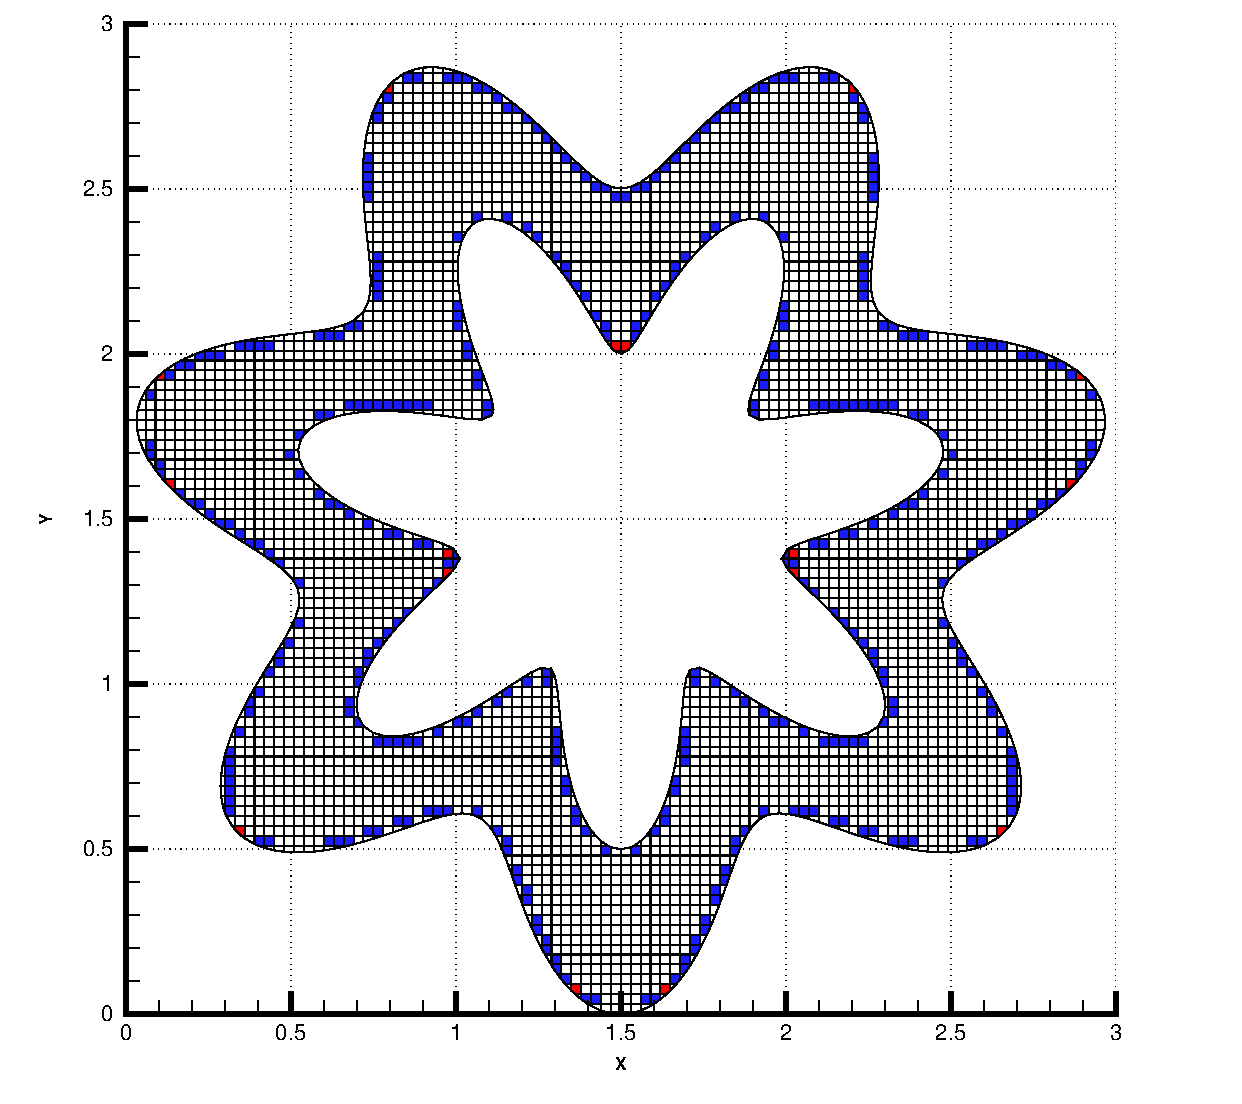
\includegraphics[width=4.5in]{figs/waveynumhoods.eps}
% \caption{\sf Domain from example XX.  Figure shows how many
% neighborhoods each cell belongs to: 
% one (white), two (blue), or three (red).
% The full example is shown in section \ref{sec:compResults}.}
% \label{fig:2nborTile}
% \end{center}
% \end{figure}

The two steps above can be part of a preprocessing step, since they do not
depend on the computed solution. For moving geometry however they would
be done at each step.
Using the merging tiles and the cell counts, the state redistribution
algorithm after one forward Euler time step is as follows:

%\begin{enumerate}[label=Step \arabic*:,leftmargin=2\parindent]
\begin{enumerate}
\item
{\bf Compute the volume-weighted and count-weighted solution for all
merged tiles.}   

\vspace*{.1in}
The contribution of each cell is divided by the number of neighborhoods 
it is part of (i.e. its count). The notation in this section refers
to cut cell $i,j$, with solution $U_{i,j}$ and volume
$V_{i,j}$. 
The provisionally updated solution before the
stabilization algorithm is applied is $\widehat{U}_{i,j}$.
There will now be many temporary merging neighborhoods which 
we denote as $\widehat{Q}_{i,j}$. 
Let $M_{i,j}$ denote the set of cell indices in the cell $(i,j)$ merging
neighborhood.  Then
\begin{equation}
\label{tiledef}
\widehat{Q}_{i,j} =  \frac{1}{{\widehat V}_{i,j}} \, \sum_{k \in M_i} \,  
\frac{V_k}{N_k}  \,\,  \widehat{U}_k
\end{equation}
where the volume ${\widehat V}_{i,j}$ is the merging tile volume similarly weighted,
\begin{equation}
\label{voldef}
{\widehat V}_{i,j} =  \sum_{k \in M_i } \,  \frac{V_k}{N_k}  .
\end{equation}

In other words, the contributions from each cell are weighted by the
number of neighborhoods they contribute to.
In the above equations, $k$ is  a multi-index ranging over the neighbors 
of cell $i,j$ included in its merging tile.
Note that most full cells will have ${\widehat V}_{i,j} = V_{i,j}$, 
and $\widehat{Q}_{i,j}  = \widehat{U}_{i,j}$.





\item
{\bf Compute a (limited) gradient for each merging
tile.}

\vspace*{.1in}
For cut cells, a least squares procedure  similar to the one used for
the finite volume update is an obvious choice. However instead of using the
solution $U_{i,j}$ on the Cartesian mesh at time $t_n$,
the merging neighborhood solution  $\widehat{Q}_{i,j}$ is used. It is important
to note that the centroid of the merging neighborhood is \textit{not} the centroid of cell ${i,j}$ (figure \ref{fig:centroids}).
\begin{figure}
    \centering
    \subfloat[]{\includegraphics[width=0.45\linewidth]{figs/centroids3.pdf}} \hfill
    \subfloat[]{\includegraphics[width=0.45\linewidth]{figs/centroids4.pdf}}
    \caption{The centroids of the Cartesian and cut cells are indicated with a solid circle ($\bullet$).  The centroids and weighted centroids of the merging neighborhoods are indicated with a square ($\blacksquare$) and a cross ($\times$), respectively. Note that the centroids and weighted centroid of the cut cell neighborhoods do not necessarily coincide.}
    \label{fig:centroids}
\end{figure}
The reconstruction neighborhood for $i,j$ is initialized to the $3 \times 3$ tile centered on $i,j$.
With this choice, it could happen that the centroids are too close to each other to compute a gradient in the normal direction (figure \ref{fig:tooclose}). If the weighted centroids are not at least $0.5\,\Delta x$  and $0.5\,\Delta y$ apart in the $x$ or $y$ direction then we increase the stencil size for the gradient computation.  For example, if the weighted centroids are too close in the $x$ direction, but not the $y$ direction, then the $5\times 3$ tile is used as the reconstruction neighborhood.  Similarly, if the weighted centroids are too close in the $y$ direction, but not the $x$ direction, then the $3\times 5$ tile is used as the reconstruction neighborhood.  The neighborhood size is increased until the distance constraint is satisfied in both directions.  In figure \ref{fig:tooclose}, the appropriate reconstruction neighborhood is $3\times 5$ reconstruction tile.
% The same neighborhood that is used for computing the gradient can be used to limit the gradient to prevent overshoots. The centroid is computed using the same weighting by number of neighborhoods as when the volume was computed. (IS THIS TRUE AND IS IT NECESSARY) NEED DISCUSSION OF NOT A REAL CENTROID
% For most full cells with a count of one, the normal gradient computation as done in the finite volume update will suffice.

\begin{figure}
    \centering
    \subfloat[]{\includegraphics[width=0.45\linewidth]{figs/tooclose2.pdf}} \hfill
    \subfloat[]{\includegraphics[width=0.45\linewidth]{figs/tooclose1.pdf}} 
    \caption{The blue cell's $3\times3$ reconstruction tile highlighted in green.  The weighted centroids are indicated with a cross ($\times$).}
    \label{fig:tooclose}
\end{figure}

\item
{\bf Replace the provisionally computed cut cell values and their adjacent
full cell neighbors with  the contributions from the merged tiles.} 

\vspace*{.1in}
The final solution at time $t^{n+1}$ on cut cell $i,j$ is obtained by compiling a the indices of all merging neighborhoods that overlap cell $i,j$ in the set $W_{i,j}$.  Then, the solution on merging neighborhood $k,l$ in $W_{i,j}$ is evaluated at $i,j$'s physical centroid, $x_{i,j}$, given by $\hat{q}_{k,l}(x_{i,j})$.  The final solution value on cell $i,j$ is given by the average of these values, i.e.,
\begin{equation} \label{eq:final_update_linear}
U^{n+1}_{i,j} := \frac{1}{N_{i,j}}\sum_{(k,l) \in W_{i,j}}\hat{q}_{k,l}(x_{i,j}).
\end{equation}
To use the example of figure \ref{fig:2nborTile}, the cut cell value
\begin{equation}
   U_{i,j}^{n+1} := \widehat{Q}_{i,j} 
   + (x_m - x_{i,j}) \, \frac{\partial \widehat{Q}_{i,j}}{\partial x} 
   + (y_m - y_{i,j}) \, \frac{\partial \widehat{Q}_{i,j}}{\partial y}
\end{equation}
since cell ${i,j}$ only belongs to one neighborhood. The adjacent full cell
on the other hand belongs to two neighborhoods -- the one it shares with
the cut cell $i,j$ , and its own merging neighborhood.
So its solution at time $t_{n+1}$  becomes
\begin{equation}
\label{eqn:numhood2ex}
\begin{split}
   U_{i,j+1}^{n+1} \,=\, & \frac{1}{2}\widehat{q}_{i,j}(x_{i,j})+ \frac{1}{2} \widehat{q}_{i,j+1}(x_{i,j}), \\
   = &\frac{1}{2} \left
   (\widehat{Q}_{i,j} 
   + (x_m - x_{i,j+1}) \, \frac{\partial \widehat{Q}_{i,j}}{\partial x} 
   + (y_m - y_{i,j+1}) \, \frac{\partial \widehat{Q}_{i,j}}{\partial y} \right ) + \frac{1}{2} \widehat{Q}_{i,j+1} .
\end{split}
\end{equation}
The last term  in eq. \eqref{eqn:numhood2ex} has no gradient terms because the
centroids of the original cell and merged cell are identical.
The fraction $\frac{1}{2}$ is because cell $(i,j+1)$ is part of  two
neighborhoods, so each contributes half of the solution.
\end{enumerate}

Different choices of neighborhoods, the minimum volume for the merging
neighborhood, gradient neighborhoods, and limiting will give
somewhat different computational results. Some of these will be examined
theoretically using model problems in one space dimension in section
\ref{sec:theory}. These choices can affect the stability limit of the
overall method.
We will also show computational results using different neighborhood
choices in section \ref{sec:compResults} in two space dimensions.

The conservation properties of the algorithm will be discussed after the
higher order SRD algorithm is presented in the next
section (PR PUT IT HERE). It will also be prseented more generally.   
OTHER THINGS HERE? DEMONSTRATE LINEARLY EXACT SECOND ORDER CONVERGENCE
HERE INSTEAD OF COMPRESULTS SECTION?

% SOMEHWERE PUT IMPLEMENTATION SUBSECTION OR AT LEAST A PARAGRAPH
% TO NOTE THAT THE CELL DOESNT KNOW WHO GIVES TO
% IT, SO THIS LOOP IS OVER GIVERS  NOT RECEIVERS.
The final update formula \eqref{eq:final_update_linear} can easily be implemented with a nested for loop in algorithm \ref{alg:finalupdate}.  
The outer loop iterates over the merging neighborhoods $i,j$ and the inner loop iterates over each cell $k,l$ in merging neighborhood $i,j$.  Each merging neighborhood $i,j$ gives a contribution $ \hat{q}_{i,j}(x_{k,l})/N_{k,l} $ to the cells $k,l$ that belong to it.
\begin{algorithm}[H]
\SetAlgoLined
$U^{n+1}(:,:) := 0$\\
 \ForAll{$i,j$}{
     \ForAll{$(k,l) \in M_{i,j}$}{
        $U^{n+1}(k,l) := U^{n+1}(k,l) + \hat{q}_{i,j}(x_{k,l})/N_{k,l} $
     }
 }
 \caption{Final solution update} \label{alg:finalupdate}
\end{algorithm}

\begin{figure}
	\subfloat[]{\includegraphics[width=0.45\textwidth]{figs/modelexample2D_1.pdf} \label{fig:2nborTile1}}
	\hfill
	\subfloat[]{\includegraphics[width=.45\textwidth]{figs/modelexample2D_2.pdf} \label{fig:2nborTile2}}
	\caption{Two-dimensional example of overlapping neighborhoods.  The unweighted centroids of cells $i,j$ and $i,j+1$ are indicated with solid squares ($\blacksquare$).} \label{fig:2nborTile}
\end{figure}


\subsection{Limiting on merging neighborhoods}
In this section we design a linearity preserving limiter for slopes on merging neighborhoods.  Designing a limiter that does not destroy the linearly preserving property is not so straightforward.  
%We demonstrate this
%In particular, we apply the LP limiter [] on slopes
\section{Computational Results}\label{compResults}

\subsection{Linear convergence study}
We solve \eqref{eq:conslaw} with the flux $\mathbf{F}(u) = [-2\pi y u, 2\pi x u]$ and initial condition
$$
u_0(x,y) = 
$$
until the final time $T = 1$ on the domain comprising two concentric discs in Figure \ref{fig:channel}.   
\subsection{Nonlinear convergence study}
\section{Conclusions}\label{sec:conc}
We have presented a  state redistribution algorithm to solve the small cell problem on cut cell meshes.  It is conservative, allows for overlapping temporary merging neighborhoods so is easy to implement, and is linearity preserving.   
Numerical experiments show that on smooth problems, second order accuracy is maintained, and the solution is not degraded by the postprocessing. For problems with shocks, the scheme maintains robustness at the cut cells.
We have shown experiments using SRD on two different base schemes, but it should be 
applicable to any underlying numerical method with
cell-centered variables.

We think that state redistribution should be applicable to 
different sets of equations, and to three-dimensional applications.
It also seems clear that the scheme can be extended to higher order accuracy, 
when used in conjunction with a 
higher order base scheme. We have already started extending this work to
3rd and 4th order accuracy. Higher order methods bring 
in many new features however, so we do not include that here.

%\section{Higher-Order State Redistribution Algorithm}\label{sec:ho}

The higher order version is essentially the same as the second order
version, but with a larger stencil so a higher order polynomial can be
reconstructed for each merging neighborhood. Of course, the base method
has to be higher order too. We use a 3rd order TVD Runge Kutta scheme
for the base method.  The spatial accuracy is improved by using a
quadratic or cubic reconstruction, taking care to translate
accurately between conservtive and primitive variables.  Higher
order polynomials are also used for reconstruction on the merged cells. 
The stability limit for the 3rd order TVD Runge-Kutta scheme with
quadratic reconstruction is
\begin{equation}
ANDREW - What is it?
\end{equation}
Again this is fairly standard, so we go right
to the description of the higher-order SRD algorithm.

\begin{enumerate}
\item 
\textbf{Compute the solution average on each merging tile}

This step is the same as the second order case.
Again using $\bar{U}_k$ to represent the provisionally updated 
solution after one step or stage, form merged solutions 
\begin{equation}\label{eq:q_avg1}
     \widehat{Q}_{ij} =  \frac{1}{ V_m}_{ij} \, \sum_{k \in
     M_i}\frac{V_k}{N_k} \bar U_k.
\end{equation}
\noindent where $M_i$ is again the set of indices of cells in the 
merging neighborhood, and the volume of the merged tile 
\begin{equation}\label{eq:modV}
{V_m}_{ij} = \sum_{k \in M_i}\frac{V_k}{N_k} .
\end{equation}

\item \textbf{Determine a polynomial reconstruction $\hat q_i(x)$ on 
each merging tile of the form}
% \begin{equation}\label{eq:q}
% \begin{aligned}
%     \hat q_(x,y) = \hat Q_{m} + \hat \sigma_{m,x}\frac{x-\hat x_m}{\Delta x} +  \hat \sigma_{m,y}\frac{y-\hat y_m}{\Delta y} + \frac{1}{2}\hat \delta_{m, xx}\left[ \frac{(x - \hat x_m)^2 }{\Delta x^2} - \hat S_{m,xx}\right]\\
% 	    +\hat \delta_{m, xy}\left[ \frac{(x - \hat x_m) (y - \hat y_m) }{\Delta x \Delta y} - \hat S_{m,xy}\right] + \frac{1}{2}\hat \delta_{m, yy}\left[ \frac{(y - \hat y_m)^2 }{\Delta y^2} -  \hat S_{m,yy}\right]\\
% 	    + \frac{1}{6}\hat\gamma_{m, xxx}\left[ \frac{(x -  \hat x_m)^3 }{\Delta x^3} -  \hat S_{m,xxx}\right] + \frac{1}{2}\hat \gamma_{m, xxy}\left[ \frac{(x - \hat x_m)^2 (y -  \hat y_m) }{\Delta x^2 \Delta y} -  \hat S_{m,xxy}\right]\\
% 	     + \frac{1}{2}\hat \gamma_{m, xyy}\left[ \frac{(x -  \hat x_m) (y -  \hat y_m)^2 }{\Delta x \Delta y ^2} -  \hat S_{m,xyy}\right]+ \frac{1}{6}\hat \gamma_{m, yyy}\left[ \frac{(y -  \hat y_m)^3 }{\Delta y^3} -  \hat S_{m,yyy}\right],
% \end{aligned}
% \end{equation}
\begin{equation}\label{eq:q}
\begin{aligned}
    \hat q (x,y) = \sum_{|\alpha| \leq p}  \frac{1}{\alpha!} (\partial^{\alpha} \hat q) [h^{\alpha}-\hat S_{m, \alpha}]
\end{aligned}
\end{equation}
where $\alpha = (\alpha_1, \alpha_2)$, $|\alpha| = \alpha_1 + \alpha_2$, $h^{\alpha} = (x-\hat x_m)^{\alpha_1}(y-\hat y_m)^{\alpha_2}$, $\partial^{\alpha} = \partial^{\alpha_1}\partial^{\alpha_2}$,
and $\hat x_m$, $\hat y_m$ is the weighted centroid of the merging
neighborhood for cell $i,j$. 
The $ \hat S_{m,\alpha}$ is a geometric
constant that make it easier to maintain conservation when written in
this form.  The reconstruction satisfies
\begin{equation}\label{eq:qi}
\frac{1}{V_m}\sum_{k \in M_j}\frac{1}{N_k}\int_{\Omega_k} \hat q_i(x)~d\Omega_k = \hat Q_j \quad \forall j \in R_i,
\end{equation}
where $R_i$ is the set of indices of neighborhoods used for reconstruction 
on merging neighborhood $i$ of the form


\item \textbf{Set the final solution at time $t^{n+1}$}
	\begin{equation}\label{eq:final_update}
	U^{n+1}_i =  \frac{1}{V_i}\sum_{k \in M_{i}}\frac{1}{N_i}\int_{\Omega_i} \hat q_k(x)~d\Omega_i,
	\end{equation}
	where $M_i$ is a set of merging tile indices to which cell $i$ belongs.
\end{enumerate}

\subsection{Limiting on merging neighborhoods}


\subsection{Conservation}\label{sec:cons}
The total mass of the numerical solution at $t^{n+1}$ is
\begin{equation}\label{eq:total_mass}
\mathcal{M}^{n+1} = \sum^N_{i=1} h_i U^{n+1}_i.
\end{equation}
From the general form of the state redistribution algorithm 
in \eqref{eqn:final_update}, 
this can also be written as a sum of mass contributions from each 
merging neighborhood, i.e.,
\begin{equation}\label{eq:total_mass2}
\mathcal{M}^{n+1} = \sum^N_{i=1} \hat{\mathcal{M}}_i,
\end{equation}
where the mass contribution of merging neighborhood $i$ is
\begin{equation}\label{eq:mi}
\hat{\mathcal{M}}_i = \sum_{k \in M_i}\frac{1}{N_k} \int_{\Omega_k}\hat q_i(x) ~d\Omega_k,
\end{equation}
and $\hat q_i(x)$ is that neighborhood's polynomial reconstruction.  
From \eqref{eq:qi}, \eqref{eq:mi} becomes
\begin{equation}\label{eq:mi1}
\hat{\mathcal{M}}_i = \hat Q_i \hat V_i.
\end{equation}
% \subsection{First order algorithm}
% When $\hat q_i(x)$ is constant, i.e. $\hat q_i(x) = \hat Q_i$ by \eqref{eq:q_avg} and Step 2 in Section \ref{sec:first_order}, \eqref{eq:mi} becomes 
% Substituting \eqref{eq:mi} into \eqref{eq:total_mass2}, we have
% \begin{equation}\label{eq:mi1}
% \hat{\mathcal{M}}_i = \hat Q_i \hat V_i.
% \end{equation}
% by \eqref{eq:q_avg} in the first order algorithm, by \eqref{eq:pq2} in the second order algorithm, and by \eqref{eq:q2} in the third order algorithm.
From \eqref{eq:modV} and \eqref{eq:q_avg1}, \eqref{eq:mi1} becomes
\begin{equation}\label{eq:mi2}
\hat{\mathcal{M}}_i = \sum^{M_i}_{k = m_i}\frac{h_k}{N_k} \hat U_{k}.
\end{equation}
Substituting \eqref{eq:mi2} into \eqref{eq:total_mass2}, the mass at $t^{n+1}$ is
$$
\mathcal{M}^{n+1} = \sum^{N}_{i=1} h_i \hat U_i,
$$
which shows that $\mathcal{M}^{n+1}  = \mathcal{M}^{n} $.

	



%\subsection*{Acknowledgments} 
%This work was supported in part by Grant Number


\newpage
\small
\bibliography{references}
\bibliographystyle{plain}



\end{document}
